\qrchapter{https://forgottenpillar.com/rsc/pl-fp-chapter3}{Kontekst Historyczny}

Ellen White wspomniała, że napotkała te same poglądy w \textit{The Living Temple}, przed którymi ostrzegała na początku swojej służby:

\egw{Podczas czytania \normaltext{[The Living Temple]} rozpoznałam te same poglądy, przed którymi miałam polecenie ostrzegać \textbf{we wczesnych dniach mojej publicznej służby}. \textbf{Kiedy po raz pierwszy opuściłam \underline{stan Maine, było to po to, by udać się przez Vermont i Massachusetts}}, aby nieść świadectwo \textbf{przeciwko tym poglądom}. «The Living Temple» zawiera alfę tych teorii. Wiedziałam, że omega nastąpi wkrótce; i drżałam o nasz lud. Wiedziałam, że muszę ostrzec naszych braci i siostry, \textbf{aby nie wdawali się w spory dotyczące \underline{obecności i osobowości Boga}}. Stwierdzenia zawarte w «The Living Temple» w tej kwestii są nieprawidłowe. Tylko przez błędne zastosowanie Pisma można poprzeć przedstawioną tam doktrynę}[SpTB02 53.2; 1904][https://egwwritings.org/read?panels=p417.271]

Dokładnie określiła, kiedy po raz pierwszy spotkała się z tymi poglądami: \egw{Kiedy po raz pierwszy opuściłam \textbf{stan Maine}, było to po to, by udać się przez Vermont i Massachusetts, \textbf{aby nieść świadectwo przeciwko tym poglądom}} Jej biografia, napisana przez jej wnuka Arthura Laceya White'a, dostarcza szerszego kontekstu dla tych poglądów. W książce \textit{Ellen White: The Early Years}, w sekcji „\textit{Wrestling with the Views of the Spiritualizers}”, jej doświadczenia we wschodnim Maine ujawniają więcej na temat sporu dotyczącego osobowości Boga i jego następstw.

\othersQuote{\textbf{\underline{We wschodnim Maine Ellen podróżowała}} i pracowała \textbf{w atmosferze spirytualistów, którzy \underline{za alegorie uznali niebo, Boga, Jezusa i nadzieję drugiego przyjścia}}. W wizji w Exeter w połowie lutego wydawało się, że \textbf{znajduje się w obecności Jezusa, i gorliwie pragnęła uzyskać odpowiedzi na niektóre \underline{istotne pytania}}}[ALW, 1BIO 79.4; 1985][https://egwwritings.org/read?panels=p668.582]

\othersQuoteNoGap{Zapytałam Jezusa, czy \textbf{Jego Ojciec ma postać jak On}. \textbf{Powiedział, że ma}, lecz nie mogłam jej ujrzeć, ponieważ powiedział: «Gdybyś choć raz ujrzała chwałę \textbf{Jego osoby}, przestałabyś istnieć». — Early Writings, str. 54}[ALW, 1BIO 79.5; 1985][https://egwwritings.org/read?panels=p668.583]

\othersQuoteNoGap{Nie była to jedyna okazja, przy której Ellen rozmawiała z Jezusem i aniołem \textbf{o \underline{osobie Jezusa} i o tym, że \underline{Bóg jest osobową istotą}}. \textbf{\underline{Odpowiedzi w pełni ją przekonały, że spirytualiści są w głębokim błędzie}}}[ALW, 1BIO 80.1; 1985][https://egwwritings.org/read?panels=p668.586]

Wizja, o której wspomniał Arthur Lacey White, znana jest jako \textit{wizja o osobowości Boga}, którą zbadamy później. Ta wizja potwierdza, że doktryna \emcap{o osobowości Boga} naucza, że Bóg Ojciec ma postać, tak jak Jezus. Odnosi się ona szczególnie do \othersnodot{\textbf{osoby Jezusa} i do tego, że \textbf{Bóg jest osobową istotą}.}

\begin{figure}[t]
    \centering
    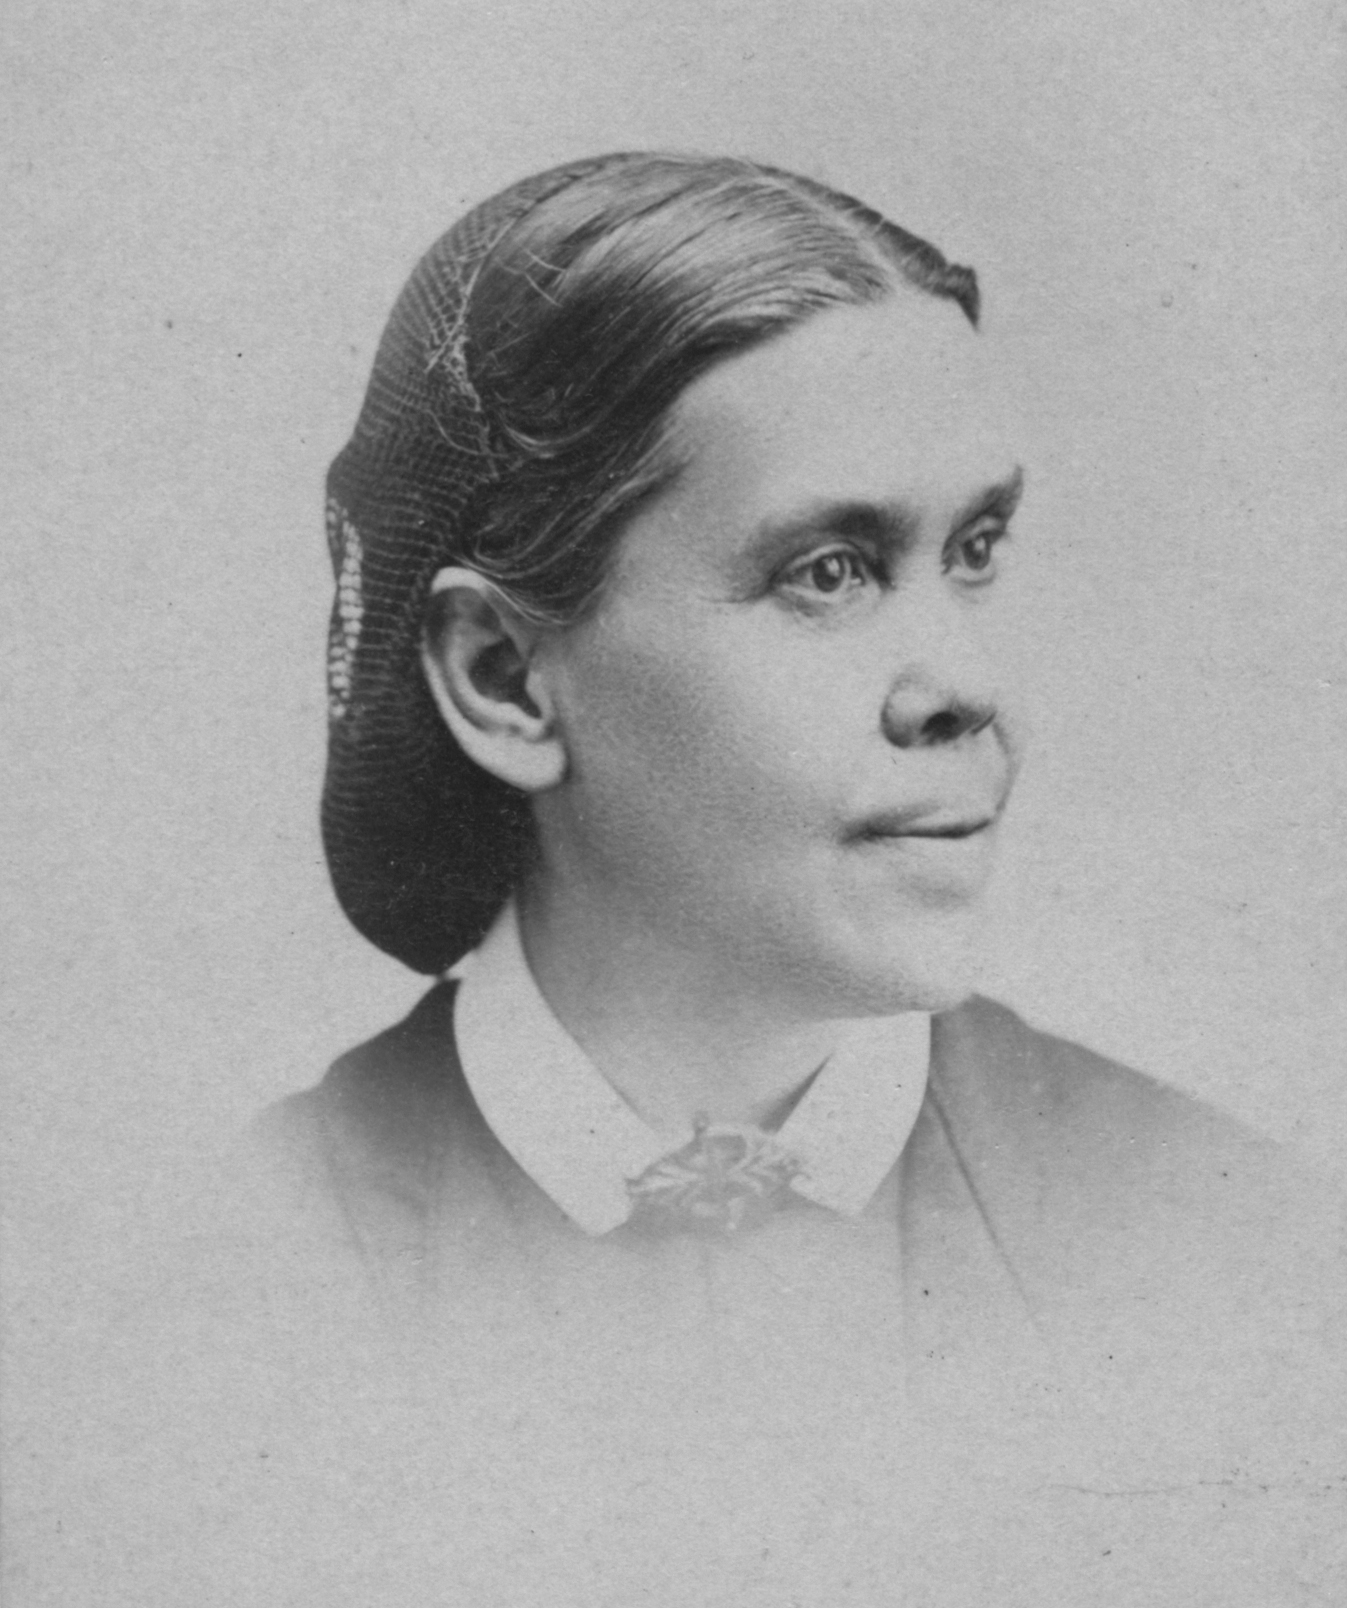
\includegraphics[width=0.65\linewidth]{images/ellen-white.jpg}
    \caption*{Ellen G. White}
    \label{fig:ellen-g-white}
\end{figure}

Rozważmy pierwszy punkt \emcap{Fundamentalnych Zasad}, który stwierdza, że Adwentyści Dnia Siódmego wierzą w \others{jednego Boga, \textbf{osobową, duchową istotę}}[First point of the Fundamental Principles][https://forgotten-pillar.s3.us-east-2.amazonaws.com/A+declaration+of+the+fundamental+principles+taught+and+practiced+by+the+Seventh-day+Adventists++.pdf] To jasno pokazuje, że główną kwestią w doktrynie \emcap{osobowości Boga} jest zewnętrzna, cielesna postać Ojca. Ale dlaczego było to tak istotne i znaczące pytanie? Jakie były implikacje tego, że Bóg ma cielesną, osobową postać?

\othersQuote{Ale ponieważ pionierzy Kościoła Adwentystów Dnia Siódmego utrzymywali, że proroctwo wypełniło się 22 października 1844 roku i że w tym czasie rozpoczęła się w niebie w Miejscu Najświętszym niebiańskiej świątyni ważna praca, i ponieważ adwentyści, którzy stali się \textbf{spirytualistami} zajęli stanowisko, że Chrystus wszedł do ich serc 22 października 1844 roku i że Jego królestwo jest w ich sercach, założyciele Kościoła, a szczególnie Ellen White, byli klasyfikowani ogólnie przez świat, a także przez tych, których ADS określali adwentystami dnia pierwszego, jako jedna i ta sama grupa. Tu znowu wielki wróg rzucił oszczerstwo na prawdę, zestawiając ją z fałszywym, rzekomym doświadczeniem}[ALW, 1BIO 80.2; 1985][https://egwwritings.org/read?panels=p668.587]

\othersQuoteNoGap{Ellen White miała mówić o tej sprawie ponownie, szczególnie w końcowych akapitach swojej pierwszej małej książki, «Experience and Views», opublikowanej w 1851 roku. Czytając to, należy zwrócić uwagę na użycie \textbf{terminu spirytualizm}, który musi być rozumiany w świetle działalności spirytualistów, a nie w świetle tego, co dziś rozumie się jako spirytualizm czy spirytyzm, chociaż oba pochodzą z tego samego źródła}[ALW, 1BIO 80.3; 1985][https://egwwritings.org/read?panels=p668.588]

\othersQuoteNoGap{Przechodzimy teraz do oświadczenia napisanego i opublikowanego w 1851 roku, które znajduje się w Ibid., 77, 78:}[ALW, 1BIO 80.4; 1985][https://egwwritings.org/read?panels=p668.589]

\othersQuoteNoGap{\textbf{Często fałszywie oskarżano mnie o nauczanie poglądów charakterystycznych dla spirytualizmu}. Ale zanim redaktor The Day-Star popadł w to złudzenie, \textbf{Pan \underline{dał mi wizję} smutnych i niszczycielskich skutków, jakie on i inni wywołają w stadzie \underline{nauczając duchowych poglądów}}.}[ALW, 1BIO 80.5; 1985][https://egwwritings.org/read?panels=p668.590]

\othersQuoteNoGap{Często widziałam kochanego \textbf{Jezusa, że jest On osobą}. Zapytałam Go, \textbf{\underline{czy Jego Ojciec jest osobą} i \underline{ma postać} jak On}. Jezus odpowiedział: «Jestem \textbf{dokładnym obrazem osoby Mojego Ojca}»}[ALW, 1BIO 80.6; 1985][https://egwwritings.org/read?panels=p668.591]

\othersQuoteNoGap{\textbf{Często widziałam, że \underline{spirytualistyczny pogląd} odebrał całą chwałę niebu, a w wielu umysłach tron Dawida i urocza osoba Jezusa zostały spalone w ogniu spirytualizmu.} Widziałam, że pewni ludzie, którzy zostali zwiedzeni i wprowadzeni w ten błąd, zostaną wyprowadzeni na światło prawdy, ale będzie prawie niemożliwe, aby całkowicie uwolnili się od \textbf{zwodniczej mocy spirytualizmu}. Tacy powinni skrupulatnie wyznać swoje błędy i na zawsze je porzucić}[ALW, 1BIO 80.7; 1985][https://egwwritings.org/read?panels=p668.592]

\othersQuoteNoGap{\textbf{Odrealnienie nieba, Boga, Chrystusa i przyjścia Chrystusa leżało u podstaw wielu fanatycznych nauk, którym siedemnastoletnia Ellen Harmon zgodnie z Bożym powołaniem miała stawić czoła w tych początkowych dniach. Wizje mocno ugruntowały \underline{osobowość Boga i Chrystusa} oraz \underline{realność nieba}, nagrody dla wiernych i zmartwychwstania. To rozsądne prowadzenie uratowało formujący się Kościół}.}[ALW, 1BIO 81.1; 1985][https://egwwritings.org/read?panels=p668.595]

Błąd ruchu Millerytów w 1844 roku polegał na niezrozumieniu natury wydarzenia, a nie jego czasu. Księga Daniela 7:13--14 opisuje Chrystusa przychodzącego do Odwiecznego w niebie, aby otrzymać władzę, chwałę i królestwo — nie Jego drugie przyjście na ziemię. To wydarzenie, oznaczające początek dzieła Chrystusa w Miejscu Najświętszym, nastąpiło na zakończenie proroctwa o 2300 dniach w 1844 roku. W przeciwieństwie do innych grup adwentystycznych rodzący się Kościół Adwentystów Dnia Siódmego w unikatowy sposób rozpoznał to niebiańskie wydarzenie.

To zrozumienie opiera się na kluczowych założeniach:
\begin{itemize}
    \item Niebo jest realnym, dosłownym miejscem (J 14:1--3).
    \item W niebie znajduje się dosłowna świątynia, w której służy Chrystus (Hbr 8:2).
    \item W tej świątyni istnieje realny, fizyczny tron, zajmowany przez samego Boga (Dn 7:9--10; Obj 4:2--3; Ez 1:26--28; Ps 11:4).
\end{itemize}

Dlaczego kwestia cielesnej postaci Ojca jest tak ważna? Gdyby Bóg nie był fizyczną istotą, nie byłoby potrzeby dosłownego tronu, świątyni ani niebiańskiej służby. Spirytualistyczna interpretacja podważa fundament teologii Adwentystów Dnia Siódmego, prowadząc do efektu domina, który niszczy doktrynę o kapłańskiej służbie Chrystusa.

Doktryna o \emcap{osobowości Boga} była prostym, ale fundamentalnym nauczaniem, potwierdzonym w pierwszym punkcie \emcap{Fundamentalnych Zasad}: \textit{„Jeden Bóg, osobowa, duchowa istota”.} Jako taki, nie jest On wszechobecny sam w sobie, ale poprzez swojego przedstawiciela, Ducha Świętego.\footnote{Pierwszy punkt Fundamentalnych Zasad: \othersQuote{Że jest \textbf{jeden Bóg}, \textbf{\underline{osobowa, duchowa istota}}, stwórca wszystkich rzeczy, wszechmocny, ... i \textbf{wszędzie obecny przez \underline{swojego przedstawiciela}, Ducha Świętego}. Ps 139:7}} Kiedy Ellen White zapytała Jezusa, \egwinline{czy Jego Ojciec \textbf{jest osobą} i \textbf{ma \underline{postać}} jak On}[EW 77.1; 1882][https://egwwritings.org/read?panels=p28.490&index=0], widzimy wyraźnie, że \textit{zewnętrzna cielesna \textbf{postać}} jest \textit{właściwością lub stanem} definiującym Boga jako osobę. To zrozumienie było kluczowe w rozwiązywaniu kryzysu Kellogga dotyczącego książki \textit{The Living Temple}, która odbiegała od tego podstawowego przekonania.

Lecz czy nasze obecne \textit{Fundamentalne Wierzenia} nadal potwierdzają tę doktrynę? Czy wyraźnie nauczają, że Bóg jest realną osobą o cielesnej postaci, której dosłowna obecność jest w niebie, podczas gdy jest On wszechobecny przez swojego Ducha? Doktryna o obecności i osobowości Boga jest nieobecna w dzisiejszych oficjalnych wierzeniach. Chociaż indywidualnie możemy nadal w to wierzyć, dlaczego tak istotne nauczanie zostało pominięte? Jakie były powody tej zmiany? To są pytania, które musimy dalej zgłębiać w kontekście \textit{Fundamentu Naszej Wiary}.

% The Historical Context
\begin{titledpoem}
    \stanza{
        Młoda Ellen przez Maine wędrowała, \\
        Przed błędnymi poglądami ostrzegała. \\
        Bóg ma postać, jak Chrystus objawił, \\
        I ten fakt w wizji Pan jej przedstawił.
    }

    \stanza{
        Spirytualista koncepcję swą sieje, \\
        Że fizyczne niebo wcale nie istnieje. \\
        Lecz osobowość Boga to nie abstrakcja pusta, \\
        To prawda, którą głosiły już pionierów usta.
    }

    \stanza{
        Alfa błędu w „Living Temple” się zjawiła, \\
        Omega wkrótce potem nastąpiła. \\
        Czy ta doktryna, niegdyś tak jasna, \\
        W naszych wierzeniach już nie wygasła?
    }
\end{titledpoem}

